\section{Theory of plasmon-pole models}
\begin{frame}
\frametitle{Self-Energy Expressions}
Given some choice of basis
\begin{align}
    &\Sigma_{pp}^{\text{corr}}(\omega) = \sum_{\mu }^{\text{RPA}}\left(\sum_{i}^{\text{occupied}} \frac{M_{pi}^{\mu }M_{ip}^{\mu }}{\omega -(\epsilon _{i}-\Omega  _{\mu })+i\eta}+ \sum_{a}^{\text{virtual}} \frac{M_{pa}^{\mu }M_{ap}^{\mu }}{\omega -(\epsilon _{a}+\Omega  _{\mu })+i\eta}\right) \\
\implies &\Sigma^c(\mathbf{k}, \omega)=\sum_{\mathbf{q}} \sum_\mu^{\mathrm{RPA}}\left(f_{\mathbf{k}-\mathbf{q}} \frac{\left|M_{\mathbf{k}, \mathbf{k}-\mathbf{q}}^\mu(\mathbf{q})\right|^2}{\omega-\varepsilon_{\mathbf{k}-\mathbf{q}}+\Omega_\mu(\mathbf{q})+i \eta}+\left[1-f_{\mathbf{k}-\mathbf{q}}\right] \frac{\left|M_{\mathbf{k}, \mathbf{k}-\mathbf{q}}^\mu(\mathbf{q})\right|^2}{\omega-\varepsilon_{\mathbf{k}-\mathbf{q}}-\Omega_\mu(\mathbf{q})+i \eta}\right)\\
&\approx \sum_{\mathbf{q}} v(q) A(q)\left[\frac{f_{\mathbf{k}-\mathbf{q}}}{\omega-\varepsilon_{\mathbf{k}-\mathbf{q}}+\tilde{\omega}(q)+i \eta}+\frac{1-f_{\mathbf{k}-\mathbf{q}}}{\omega-\varepsilon_{\mathbf{k}-\mathbf{q}}-\tilde{\omega}(q)+i \eta}\right]
\end{align}
\end{frame}
\begin{frame}
\frametitle{Where PPMs come from?}
The requirements are
\begin{equation}
\operatorname{Re} \varepsilon^{-1}(\mathbf{q}, \omega) \approx 1+\frac{\Omega^2(\mathbf{q})}{\omega^2-\tilde{\omega}^2(\mathbf{q})}
\end{equation}
and
\begin{equation}
    \operatorname{Im} \varepsilon^{-1}(\mathbf{q},\omega ) =A(\mathbf{q})\left\{\delta\left[\omega-\widetilde{\omega}(\mathbf{q})\right]-\delta\left[\omega+\widetilde{\omega}(\mathbf{q})\right]\right\}.
\end{equation}
\pause
Clearly, these expressions are only defined with a parameterization. I explore that of Hybertsen and Louie in 1986 and then also of Godby and Needs in 1985. 
\end{frame}
\begin{frame}
\frametitle{Hybertsen and Louie (1986)}
\begin{align}
   \left\{\begin{array}{l}\Omega_{G G^{\prime}}^2(q)=\omega_p^2 \frac{(q+G) \cdot\left(q+G^{\prime}\right)}{|q+G|^2} \frac{n\left(G-G^{\prime}\right)}{n(0)}\overset{UEG}{=}\omega _p^2 = 4\pi n \\ \tilde{\omega}_{G G^{\prime}}^2(q)=\frac{\Omega_{G G^{\prime}}^2(q)}{\delta_{G G^{\prime}}-\varepsilon_{G G^{\prime}}^{-1}(q, \omega=0)} \overset{UEG}{=} \frac{4\pi n}{1-\varepsilon^{-1}(q, \omega=0)}
\\ A_{G G^{\prime}}(q)=-\frac{\pi}{2} \frac{\Omega_{G G^{\prime}}(q)}{\tilde{\omega}_{G G^{\prime}}(q)} .\end{array}\right. 
\end{align}
\pause
These fulfill
\begin{equation}
    \epsilon_{\mathbf{G G}^{\prime}}^{-1}(\mathbf{q} ; 0) = \delta_{\mathbf{G G}^{\prime}} + (2/\pi) \mathrm{P} \int_0^{\infty} d \omega \omega^{-1} \operatorname{Im}_{\mathbf{G G}^{\prime}}^{-1}(\mathbf{q} ; \omega)
\end{equation}
\pause
and
\begin{equation}
    \int_0^{\infty} d \omega \omega \operatorname{Im} \epsilon_{G G^{\prime}}^{-1}(\mathrm{q} ; \omega) = -\frac{\pi}{2} \omega_p^2 \frac{\rho\left(\mathrm{G}-\mathrm{G}^{\prime}\right)}{\rho(0)} \frac{(\mathrm{q}+\mathrm{G}) \cdot\left(\mathrm{q}+\mathrm{G}^{\prime}\right)}{\mid \mathrm{q}+\mathrm{G}^2}
\end{equation}
\end{frame}
\begin{frame}
\frametitle{Godby and Needs (1985)}
\begin{align}
    \left\{\begin{array}{l}
A_{\boldsymbol{G} \boldsymbol{G}^{\prime}}(\boldsymbol{q})=\varepsilon_{\boldsymbol{G} \boldsymbol{G}^{\prime}}^{-1}(\boldsymbol{q}, \omega=0)-\delta_{\boldsymbol{G} \boldsymbol{G}^{\prime}} \\
\tilde{\omega}_{\boldsymbol{G} \boldsymbol{G}^{\prime}}^2=\omega_p^2\left[\frac{A_{\boldsymbol{G} \boldsymbol{G}^{\prime}}(\boldsymbol{q})}{\varepsilon_{\boldsymbol{G} \boldsymbol{G}^{\prime}}^{-1}(\boldsymbol{q}, \omega=0)-\varepsilon_{\boldsymbol{G} \boldsymbol{G}^{\prime}}^{-1}\left(\boldsymbol{q}, i \omega_p\right)}-1\right] \\
\Omega_{\boldsymbol{G} \boldsymbol{G}^{\prime}}^2(\boldsymbol{q})=-A_{\boldsymbol{G} \boldsymbol{G}^{\prime}}(\boldsymbol{q}) \tilde{\omega}_{\boldsymbol{G} \boldsymbol{G}^{\prime}}^2(\boldsymbol{q})
\end{array}\right.
\end{align}
\end{frame}
\section{PPMs in practice}
\begin{frame}
\frametitle{How to apply these formulas in my study? }
Here we have $\mathbf{G} = \mathbf{G}'$ and $\mathbf{q} = 0$.
\pause
 In the first implementation of GW in the Gaussian basis, they wrote
\begin{align}
    \bm{\epsilon}(\mathbf{q}, \omega) = \begin{pmatrix}
        h_{00} & w_{P 0}^{\dagger}\\
w_{P 0} & B_{P Q}
    \end{pmatrix}
\\
\implies
    \bm{\epsilon}^{-1}(\mathbf{q}, \omega) = \begin{pmatrix}
        1/h_{00} & 0\\
0 & 1/B_{P Q}
    \end{pmatrix}
\label{inv_diel}
\end{align}
\pause
Auxiliary dimension as the number of momentum transfer vectors.
\end{frame}
\begin{frame}
\frametitle{Debugging Steps}
\begin{enumerate}
    \item \textcolor{green}{%
        Can build $\chi_{\mathrm{RPA}}(\mathbf{q}, \omega)$ as sum over Casida poles 
        or via explicit inversion
        $\chi_{\mathrm{RPA}} = \dfrac{\chi_0}{1 - v \chi_0}$}\pause
\item Verify that eqn. \ref{inv_diel} reproduces this too.\pause
    \item Plot PPM forms for $\boldsymbol{\epsilon}^{-1}(\mathbf{q}, \omega)$ vs. $1 - v \chi_{\mathrm{RPA}}(\mathbf{q}, \omega)$ for a given $\mathbf{q}$. \pause
    \item Plot PPM forms for $\Sigma^c(\mathbf{k}, \omega)$ vs. the exact answer for a given $\mathbf{k}$. \pause
    \item Garnet's spectral functions should be reproduced. \textcolor{yellow}{Should we be able to do this with and without finite size corrections? }
\end{enumerate}
\end{frame}
\begin{frame}
\frametitle{Inverse dielectric plots}
\begin{figure}
    \centering
    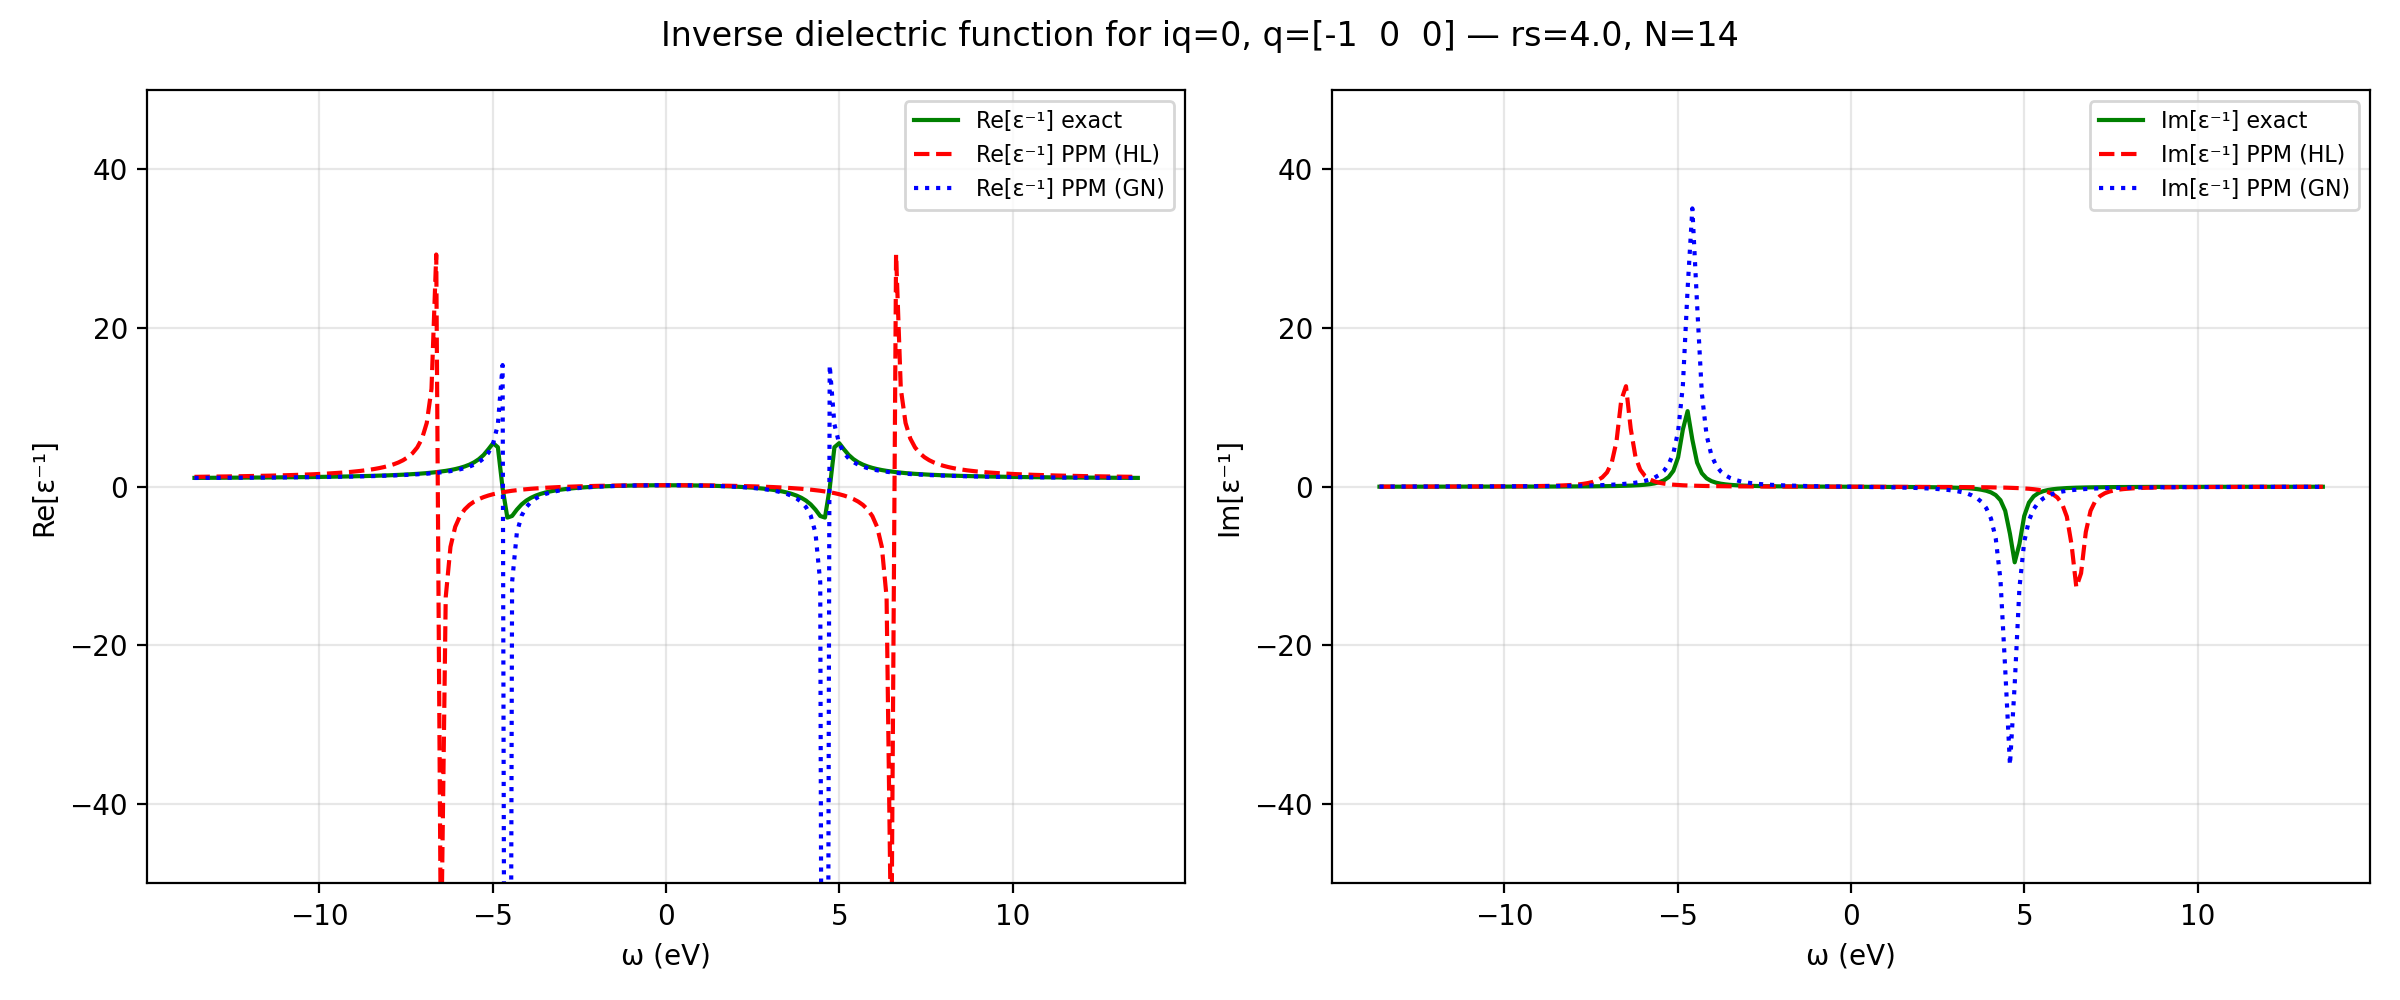
\includegraphics[width=\textwidth]{figs/inverse_dielectric_q0_rs4.png}
\end{figure}
\end{frame}
\begin{frame}
\frametitle{self energy plots}
\begin{figure}
    \centering
    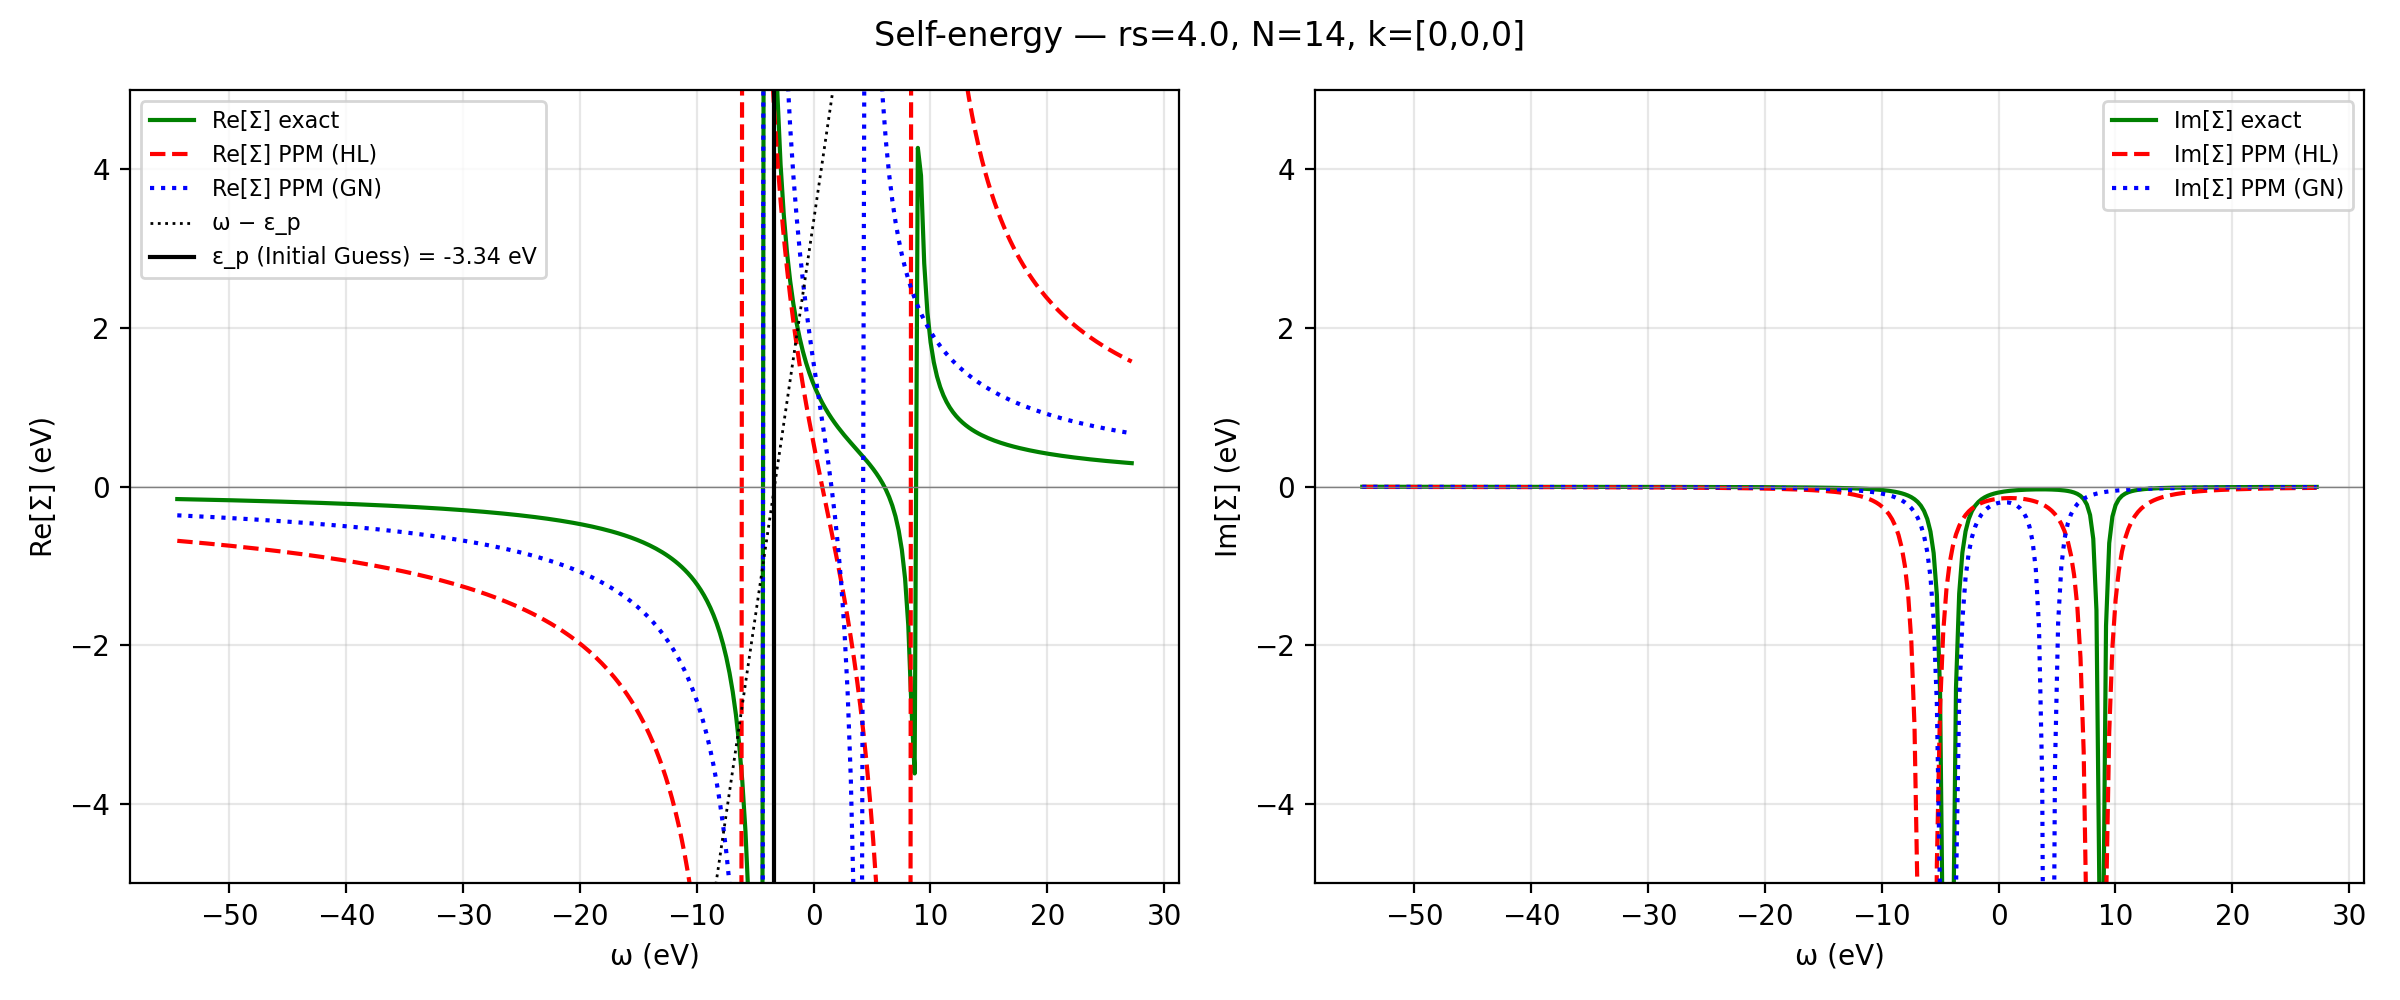
\includegraphics[width=\textwidth]{figs/selfenergy_rs4.0_pidx0.png}
\end{figure}
\end{frame}